\chapter{Numerical Characterization of Acoustic Radiation Force Impulse Imaging}
	\label{chap:arfi}
	\section{Introduction}
		Acoustic radiation force impulse imaging presents a chief benefit over quasi-static ultrasound elastography in that since the external deformation force is applied by the transducer itself rather than through manual indentation of the transducer by the diagnostician, the inter-operator reliability may be greatly increased. The net effect of this is an expected decrease in the required amount of training of diagnosticians as well as an expected increase in the sensitivity and specificity of early deep tissue injury detection.

	\section{Method}
	\label{sec:arfi_methods}
		In order to numerically characterize acoustic radiation force impulse imaging for the early detection of deep tissue injuries, a combinatory model of acoustic radiation force simulations and time-domain finite-element models of tissue deformation were used. Acoustic radiation force distributions were calculated using a k-space pseudospectral model of ultrasonic acoustics which simulated the acoustic intensities and subsequent radiation force developed by an ultrasonic transducer applying deep body loads to soft tissue. These forces were then combined with a temporal finite-element model of tissue deformation to model the response of the tissue to the body force impulses generated by the transducer. The use of these models allowed extensive simulation and parameter sensitivity analysis in order to numerically characterize the use of 

		\subsection{K-Space Pseudospectral Model of Acoustic Fields}
		\label{subsec:kspace_model}
			In order to simulate the body loads generated within deep tissue by a continuous ultrasound beam, a k-space pseudospectral model of acoustic field intensities was generated. The body load fields that were generated as a result of this model were fed into a temporal soft tissue deformation model to investigate the dynamic response of tissue to ARFI loads.

			The governing equations used for the k-space pseudospectral model were the set of coupled first-order partial differential equations \ref{equ:arfi_gov_p1} -- \ref{equ:arfi_gov_p3}. These equations are the first-order equivalents of the wave equation given in equation \ref{equ:wave_equation} taking into account acoustic absorption, tissue heterogeneities, and acoustic wave non-linearities \cite{treeby12}. Equations \ref{equ:arfi_gov_p1}, \ref{equ:arfi_gov_p2}, and \ref{equ:arfi_gov_p3} represent the momentum conservation, mass conservation, and pressure-density relation terms respectively.

			\begin{subequations}
				\label{equ:arfi_gov}
				\begin{align}
					\frac{\partial \vec{u}}{\partial t} &= - \frac{1}{\rho_0} \nabla p \label{equ:arfi_gov_p1} \\
					\frac{\partial p}{\partial t} &= -\left(2 \rho + \rho_0\right)\nabla \cdot \vec{u} - \vec{u} \cdot \nabla \rho_0 \label{equ:arfi_gov_p2} \\
					p &= c_0^2 \left(\rho + \vec{d} \cdot \nabla \rho_0 + \frac{B}{2A} \frac{\rho^2}{\rho_0} - \mathbf{L}\rho \right) \label{equ:arfi_gov_p3}
				\end{align}
			\end{subequations}

			\note[KH]{Talk about all the parameters in these equations}

			\begin{equation}
				\label{equ:wave_equation}
				\nabla^2 p - \frac{1}{c_0^2}\frac{\partial^2 p}{\partial t^2} = 0
			\end{equation}

			The $\mathbf{L}$ operator used in equation \ref{equ:arfi_gov_p3} accounts for acoustic absorption and dispersion which follows a frequency power law and is defined as per equations \ref{equ:Lop1} -- \ref{equ:Lop3}.

			\begin{subequations}
				\begin{align}
					\mathbf{L} &= \tau \frac{\partial}{\partial t}\left(-\nabla^2\right)^{\frac{y}{2} - 1} + \eta \left(-\nabla^2\right)^{\frac{y+1}{2} - 1} \label{equ:Lop1} \\
					\tau &= -2\alpha_0 c_0^{y-1} \label{equ:Lop2} \\
					\eta &= 2\alpha_0c_0^y\tan\left(\frac{\pi y}{2}\right)  \label{equ:Lop3}
				\end{align}
			\end{subequations}

			In order to integrate pressure sources in equations \ref{equ:arfi_gov_p1} -- \ref{equ:arfi_gov_p3}, equation \ref{equ:arfi_gov_p2} is modified to include a mass source term, $S_M$ which counts as a pressure source term through changing density to form equation \ref{equ:arfi_gov_p2_source}.

			\begin{equation}
				\label{equ:arfi_gov_p2_source}
				\frac{\partial p}{\partial t} = -\left(2 \rho + \rho_0\right)\nabla \cdot \vec{u} - \vec{u} \cdot \nabla \rho_0 + S_M
			\end{equation}

			The k-Wave MATLAB\textsuperscript{\textregistered} toolbox version 1.0 was used to solve for the time-variant intensities resulting from simulated acoustic radiation force impulses applied to heterogeneous soft tissue using equations \ref{equ:arfi_gov_p1}, \ref{equ:arfi_gov_p2_source}, and \ref{equ:arfi_gov_p3}. Sample source code for performing these simulations using the k-Wave toolbox is given in listing \ref{lst:intensity} in Appendix \ref{app:source_code}.

		\subsection{Derivation of Acoustic Radiation Force}
		\label{subsec:body_load_derivation}
			Acoustic radiation force arises as the result of absorption of linear momentum within tissue as acoustic waves travel though it with the requirement that the tissue is a viscoelastic medium---no energy would be absorbed in a purely linear elastic model. Further, at the super-\si{\MHz} frequencies involved in ultrasound interrogation, tissue may be considered a viscous fluid \note[KH]{Add citation!}.

			\comment{For a linearly viscous fluid, the constitutive relationship is given in equation \ref{equ:constitutive_linear_viscous} where $D_{ij}$ is defined as per equation \ref{equ:rate_deformation_linear_viscous} and represents the rate of deformation.

			\begin{equation}
				\label{equ:constitutive_linear_viscous}
				\sigma_{ij} = -p \delta_{ij} + \lambda_f D_{ii} \delta_{ij} + 2 \mu_f D_{ij}
			\end{equation}

			\begin{equation}
				\label{equ:rate_deformation_linear_viscous}
				D_{ij} = \frac{1}{2}\left(v_{i,j} + v_{j,i}\right)
			\end{equation}

			\note[KH]{Describe symbols!}

			Beginning with the Navier-Stokes equation for an incompressible Newtonian fluid given in equation \ref{equ:navier_stokes}, the acoustic radiation force may be derived given that $\mu_f$ in equation \ref{equ:navier_stokes} represents an energy loss related the an attenuation coefficient, $\alpha$ \cite{kino87}.

			\begin{equation}
				\label{equ:navier_stokes}
				-p_{,i} + \mu_f v_{i,jj} + \rho b_i = \rho\left(\dot{v_i} + v_j v_{i,j}\right)
			\end{equation}}

			Using a perturbative expansion of equation \ref{equ:arfi_linear_momentum}, acoustic radiation force can be expressed as per equations \ref{equ:radiation_force_1} \cite{nyborg65}. In equations \ref{equ:radiation_force_1}, $\langle\rangle$ represents the time-average operator, $\vec{v_1}$ and $\vec{v_2}$ are the first and second order terms in the perturbative expansion of particle velocity, and $p_2$ is the second order pressure term in the perturbative expansion, while $\vec{F}$ represents the acoustic radiation force developed in the tissue.

			\begin{equation}
				\label{equ:arfi_linear_momentum}
				\sigma_{ij,j} + \rho b_i = \rho f_i
			\end{equation}

			\begin{subequations}
				\label{equ:radiation_force_1}
				\begin{align}
					\vec{F} &= \nabla p_2 - \mu_f \nabla^2 \vec{v_2} \label{equ:radiation_force_1a} \\
					\vec{F} &= \rho \langle\vec{v_1}\nabla\cdot\vec{v_1} + \vec{v_1}\nabla\vec{v_1}\rangle \label{equ:radiation_force_1b}
				\end{align}
			\end{subequations}

			For a plane wave, equation \ref{equ:radiation_force_1b} can be reduced to equation \ref{equ:radiation_force_2}. Further, substituting the generalized wave particle velocity solution given in equation \ref{equ:particle_velocity} in equation \ref{equ:radiation_force_2}, the magnitude of acoustic radiation force may be calculated as per equation \ref{equ:radiation_force_3}.

			\begin{equation}
				\label{equ:radiation_force_2}
				\vec{F} = 2\rho\langle \vec{v} \vec{v}_{,x} \rangle
			\end{equation}

			\begin{equation}
				\label{equ:particle_velocity}
				\vec{v} = i\omega A e^{-\alpha x + i\left(\omega t - k x\right)}\hat{x}
			\end{equation}

			\begin{equation}
				\label{equ:radiation_force_3}
				\left|\vec{F}\right| = A^2 e^{-2\alpha x}\rho\alpha
			\end{equation}

			Further using the acoustic field intensity, the acoustic radiation force may be calculated as per equation \ref{equ:radiation_force} where $\alpha$ is the absorption coefficient of the tissue in \si{\neper\per\m}, $I$ is the temporal average acoustic intensity in \si{\W\per\m\squared}, and $c$ is the longitudinal speed of sound in the tissue in \si{\m\per\s} \cite{palmeri05}.

			\begin{equation}
				\label{equ:radiation_force}
				\left|\vec{F}\right| = \frac{2\alpha I}{c}
			\end{equation}

			Once acoustic radiation force body loads were calculated as per equation \ref{equ:radiation_force}, they were used as initial conditions to the temporal finite-element model of soft tissue deformation described in Section \ref{subsec:temporal_fea_arfi}.

		\subsection{Temporal Finite-Element Model of Soft Tissue Deformation}
			\label{subsec:temporal_fea_arfi}
			In response to the relatively short duration (``impulse'') acoustic radiation force body load applied to tissue in ARFI imaging, the interrogated tissue will exhibit a dynamic response---namely that tissue deformation will propagate outwards as the absorbed acoustic energy diffuses through the soft tissue.

			In order to simulate the dynamic tissue deformation generated by the acoustic impulse force, a generalized Maxwell viscoelastic model of tissue deformation was used \cite{then12}. The simulated tissue properties are summarized in Tables \ref{tab:arfi_properties} and \ref{tab:arfi_maxwell_properties}.

			\begin{table}[!htb]
				\centering
				\caption{ARFI Model Viscoelastic Tissue Properties}
				\label{tab:arfi_properties}
				\begin{tabular}{lrs[table-unit-alignment = left]}
					\toprule
					Property & Value & Units \\
					\midrule
					Bulk Modulus & 515.7 & \si{\kPa} \\
					Shear Modulus & 1.0 & \si{\kPa} \\
					Density & 1060 & \si{\kg\per\m\cubed} \\
					\bottomrule
				\end{tabular}
			\end{table}

			\begin{table}[!htb]
				\centering
				\caption{ARFI Maxwell Model Tissue Properties}
				\label{tab:arfi_maxwell_properties}
				\begin{tabular}{lrr}
					\toprule
					Branch & Shear Modulus & Relaxation Time \\
					& (\si{\Pa}) & (\si{\s}) \\
					\midrule
					1 & 791.0 & 2 \\
					2 & 66.5 & 40 \\
					3 & 0.6 & 80 \\
					\bottomrule
				\end{tabular}
			\end{table}

			% 1 791 2
			% 2 66.5 40
			% 3 0.628 80

			%the time-dependent displacement field was calculated according to equation \ref{fea:time_deformation} where \note[KH]{Don't leave us hanging!}.
			\comment{The time-dependent displacement fields were calculated according to equations \ref{fea:time_deformation} where $\sigma$ is the Cauchy stress tensor, $\vec{F}$ are the applied body forces, $\vec{u}$ is the particle displacement, $S_0$ is the initial stress distribution, $p_w$ is ?, $\vec{I}$ is the identity matrix, $G$ the shear modulus, $q_m$ is an auxiliary strain variable used to represent the extension of the $m$-th abstract string, $varepsilon$ is strain, and $t$ is time. Lesions were modeled identically to the rest of the soft tissue with the exception of the bulk and shear moduli being some fraction or multiple of the ``healthy'' moduli.

			\begin{subequations}
				\label{fea:time_deformation}
				\begin{align}
					\vec{F} &= \rho \ddot{\vec{u}} - \nabla \cdot \sigma \\
					\sigma - S_0 &= - p_w \vec{I} + 2 G\left(\varepsilon - \varepsilon_0 - \frac{1}{3} tr(\varepsilon - \varepsilon_0)\vec{I}\right) + \sum_{m=1}^N 2G_m q_m \\
					\dot{q}_m + \frac{1}{\tau_m} q_m &= \frac{\partial}{\partial t}\left(\varepsilon - \varepsilon_0 - \frac{1}{3} tr(\varepsilon - \varepsilon_0)\vec{I}\right)
				\end{align}
			\end{subequations}}

			The time-dependent displacement fields were calculated according to equation \ref{fea:time_deformation} where $\sigma$ is the Cauchy stress tensor, $\vec{F}$ are the applied body forces, and $\vec{u}$ is the particle displacement, and $\rho$ is the density.

			\begin{equation}
				\label{fea:time_deformation}
				%\vec{F} = \rho \ddot{\vec{u}} - \nabla \cdot \sigma
				\rho \frac{\partial^2 \vec{u}}{\partial t^2} - \nabla \cdot \sigma = \vec{F}
			\end{equation}

			In order to include viscoelastic effects through a generalized Maxwell model of soft tissue, equation \ref{fea:time_deformation_visco} was used where $\sigma_0$ is the initial stress distribution in the tissue, $C$ is the $4^{\text{\tiny th}}$ order elasticity tensor, $\varepsilon$ is the strain, $G_m$ and $\tau_m$ are the shear modulus and relaxation time of the $m^{\text{\tiny th}}$ branch of the Maxwell model respectively, and $\gamma_m$ is an additional auxillary degree of freedom used to represent the extension of the abstract springs in the Maxwell model.

			\begin{equation}
				\label{fea:time_deformation_visco}
				\sigma - \sigma_0 = C : \varepsilon + \sum_m 2 G_m \tau_m \dot{\gamma}_m 
			\end{equation}

			In the simulations, the boundary equations \ref{equ:arfi_fea_fixed_bc} were used to apply a fixed boundary condition to the both the bottom (deep) and top (superficial) boundaries of the model in the axial direction at both boundaries and in the lateral direction at the deep boundary. All other boundaries of the model were free to translate in all dimensions. The acoustic radiation force was applied as a body load to the tissue in the model with the distribution calculated by the k-space pseudospectral model and resultant body forces described in Sections \ref{subsec:kspace_model} and \ref{subsec:body_load_derivation}. In order to prevent reflections from the model boundaries that might affect the simulation results, the model geometry extended laterally by \SI{5}{\cm} in either direction from the centerline. Simulations were run until the axial displacement at the focal point returned to \SI{1}{\percent} of it's maximal value during the entire simulation---at this point, the tissue was considered to be ``relaxed'' after being disturbed by the acoustic radiation force.

			\begin{subequations}
				\label{equ:arfi_fea_fixed_bc}
				\begin{align}
					\vec{u} &= 0, \qquad \Gamma = \Gamma_{bottom} \\
					u_y &= 0, \qquad \Gamma = \Gamma_{top}
				\end{align}
			\end{subequations}

		\subsection{Characterizing Acoustic Radiation Force Impulse Imaging}
			%In order to fully understand the suitability of using ARFI imaging to detect and monitor deep tissue injuries, 5 general models of deep tissue injury lesions were modeled. Each general model was also investigated over a range of parameters in order to determine the relationship between the detection sensitivity and the various parameters that were studied. The investigated models included a model with hard boundaries

			\begin{figure*}[!htb]
				\centering
				\subfloat[]{
					\begin{tikzpicture}[x=0.045\textwidth, y=0.045\textwidth, draw=black, text=black, fill=black]
						% the main domain area
						\draw[fill=tissueColour] (0, 0) rectangle(10, 10);

						% the lesion
						\draw[fill=lesionColour] (7, 6) circle(0.5);

						% the lesion center marks
						\draw (6.4, 6) -- (6.9, 6);
						\draw (7.1, 6) -- (7.6, 6);
						\draw (6.95, 6) -- (7.05, 6);
						\draw (7, 5.4) -- (7, 5.9);
						\draw (7, 6.1) -- (7, 6.6);
						\draw (7, 5.95) -- (7, 6.05);

						% the lesion radius
						\draw[<-] (7.3536, 5.6464) -- (8, 5);
						\draw (7.85, 5) node[right]{\scriptsize $\diameter S$};

						% the lesion depth
						\draw (6, 6) -- (6.5, 6);
						\draw[<-] (6.25, 10) -- (6.25, 8.25);
						\draw (6.25, 8) node{\scriptsize $d$};
						\draw[->] (6.25, 7.75) -- (6.25, 6);

						% the lesion offset
						\draw (7, 5.5) -- (7, 5);
						\draw[<-] (5, 5.25) -- (5.5, 5.25);
						\draw[->] (6.5, 5.25) -- (7, 5.25);
						\draw (6, 5.25) node{\scriptsize $d_{off}$};

						% the centerline
						%\draw (5, -0.1) -- (5, 4.5);
						%\draw (5, 4.6) -- (5, 5.4);
						%\draw (5, 5.5) -- (5, 10.1);
						\draw (5, 0) -- (5, 1.9);
						\draw (5, 1.95) -- (5, 2.05);
						\draw (5, 2.1) -- (5, 3.9);
						\draw (5, 3.95) -- (5, 4.05);
						\draw (5, 4.1) -- (5, 5.9);
						\draw (5, 5.95) -- (5, 6.05);
						\draw (5, 6.1) -- (5, 7.9);
						\draw (5, 7.95) -- (5, 8.05);
						\draw(5, 8.1) -- (5, 10);

						% the domain width
						\draw (0, 10.1) -- (0, 10.5);
						\draw[<-] (0, 10.25) -- (4.25, 10.25);
						\draw (5, 10.25) node{\scriptsize \SI{10}{\cm}};
						\draw[->] (5.75, 10.25) -- (10, 10.25);
						\draw (10, 10.1) -- (10, 10.5);

						% the domain depth
						\draw (10.1, 0) -- (11, 0);
						\draw[<-] (10.75, 0) -- (10.75, 4.75);
						\draw (10.75, 5) node{\scriptsize \SI{10}{\cm}};
						\draw[->] (10.75, 5.25) -- (10.75, 10);
						\draw (10.1, 10) -- (11, 10);

					\end{tikzpicture}
					\label{fig:shear_schematic_single}
				}
				~
				\subfloat[]{
					\begin{tikzpicture}[x=0.045\textwidth, y=0.045\textwidth, draw=black, text=black, fill=black]
						% the main domain area
						\draw[fill=tissueColour] (0, 0) rectangle(10, 10);

						% the lesion
						\draw (7, 6) node{
\includegraphics[width=0.045\textwidth]{assets/shear/images/blurredLesion.png}};
						\draw (7, 6) circle(0.5);

						% the lesion radius
						\draw[<-] (7.3536, 5.6464) -- (8, 5);
						\draw (7.85, 5) node[right]{\scriptsize $\diameter S$};

					\end{tikzpicture}
					\label{fig:shear_schematic_blur}
				}
				
				\subfloat[]{
					\begin{tikzpicture}[x=0.045\textwidth, y=0.045\textwidth, draw=black, text=black, fill=black]
						% the main domain area
						\draw[fill=tissueColour] (0, 0) rectangle(10, 10);

						% the lesion
						\draw (7, 6) node{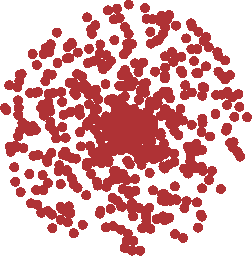
\includegraphics[width=0.045\textwidth]{assets/shear/images/clusteredLesion.png}};
						\draw (7, 6) circle(0.5);

						% the lesion radius
						\draw[<-] (7.3536, 5.6464) -- (8, 5);
						\draw (7.85, 5) node[right]{\scriptsize $\diameter S$};

						% blob size
						\draw[<-] (6.9, 5.9) -- (6, 5) node[left]{\scriptsize $r_{bl}$};

					\end{tikzpicture}
					\label{fig:shear_schematic_clustered}
				}
				~
				\subfloat[]{
					\begin{tikzpicture}[x=0.045\textwidth, y=0.045\textwidth, draw=black, text=black, fill=black]
						% the human stuffz
						\draw (5, 5) node{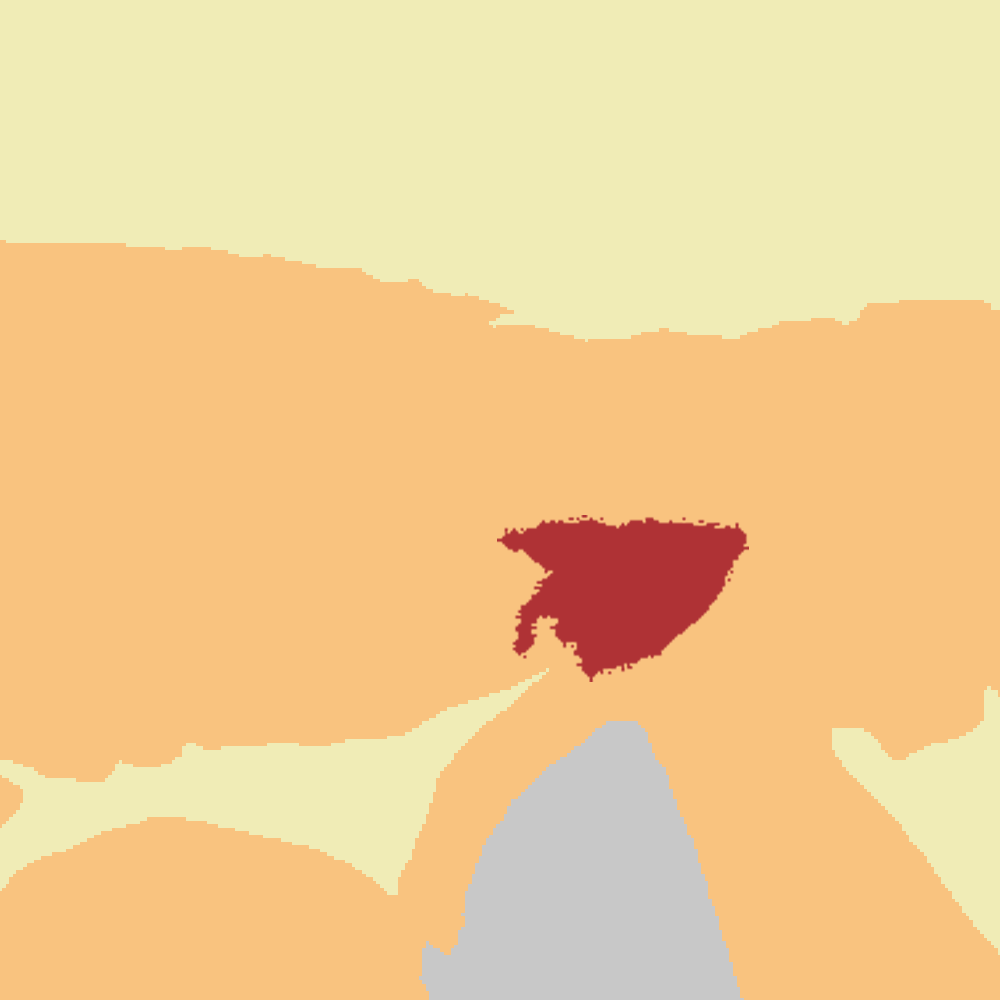
\includegraphics[width=0.45\textwidth]{assets/shear/images/humanSchematic.png}};

						% the main domain area
						\draw (0, 0) rectangle(10, 10);

						% the depth
						\draw (7.25, 4) -- (8, 4);
						\draw (7.75, 7) node{\scriptsize $d$};
						\draw[<-] (7.75, 10) -- (7.75, 7.25);
						\draw[->] (7.75, 6.75) -- (7.75, 4);

						% the size
						\draw (5, 4.7) -- (5, 5.5);
						\draw (7.25, 4.7) -- (7.25, 5.5);
						\draw (6.125, 5.25) node{\scriptsize $\diameter S$};
						\draw[<-] (5, 5.25) -- (5.75, 5.25);
						\draw[->] (6.5, 5.25) -- (7.25, 5.25);

					\end{tikzpicture}
					\label{fig:shear_schematic_human}
				}
				\caption[Schematic of shear wave speed quantification-investigated lesions]{Schematics of the lesion models that were investigated using shear wave speed quantification showing \protect\subref{fig:shear_schematic_single} a spherical hard-boundaried lesion, \protect\subref{fig:shear_schematic_blur} a spherical blurred-boundary lesion, \protect\subref{fig:shear_schematic_clustered} a cluster of numerous small lesions composing a larger lesionous region, and \protect\subref{fig:shear_schematic_human} the geometry from an MRI-acquired deep tissue injury overlaid on a slice from the Visible Human Project such that the injury lesion was located immediately superior to an ischial tuberosity.}	
				\label{fig:shear_schematics}
			\end{figure*}

			\begin{table}[!htb]
				\centering
				\caption[ARFI model investigated parameters]{Range of values of investigated parameters}
				\label{tab:arfi-parametervalues}
				\begin{tabular}{lcc}
					\toprule
					Parameter & Symbol & Values \\
					\midrule
					\bottomrule
				\end{tabular}
			\end{table}

		\subsection{Physical Phantom Validation}
			The same CIRS Elasticity QA Phantom model 049 that was used in the quasi-static studies described in Chapter \ref{chap:quasi-static} was used to experimentally validate a subset of the ARFI simulations described here. Using a Siemens ACUSON S2000 \note[KH]{Correct naming / registered marks / etc?} portable ultrasound machine with a Siemens 9L4 \note[KH]{Describe probe better}, ARFI images were acquired of lesions within the phantom. \note[KH]{More?}

	\section{Results}
		Using the k-space pseudospectral model of ultrasound acoustics described in Section \ref{subsec:kspace_model}, acoustic radiation force distributions were acquired and analyzed for a range of input parameters. These force distributions were then fed into the time-domain finite-element model of soft tissue deformation described in Section \ref{subsec:temporal_fea_arfi} to examine the difference in relationships between the true and measured tissue stiffness ratios due to the various lesion and transducer parameters listed in Table \ref{tab:arfi-parametervalues}. The results obtained through this methodology were then compared to ARFI images taken with a commercial ultrasound machine. \note[KH]{This is terrible.}

		\subsection{K-Space Pseudospectral Models of Acoustic Radiation Force}
		\label{subsec:kspace_results}
			\begin{figure}[!htb]
				\centering
				\subfloat[]{
					\begin{tikzpicture}
						\begin{axis}[
							scale only axis,
							enlargelimits=false,
							unit vector ratio*=1 1 1,
							height=3in,
							y dir=reverse,
							xlabel={X-Coordinate, $x$ (\si{\cm})},
							ylabel={Depth, $d$ (\si{\cm})},
							axis on top,
							colormap name={RdBu},
							colorbar, point meta min=-175, point meta max=175, colorbar style={at={(1.05,0)}, anchor=south west, width=0.03\textwidth, ylabel={Acoustic Radiation Force, $F_{ARFI}$ (\si{\kN\per\metre\cubed})},
							draw=black, text=black, fill=black}]
								\addplot graphics[xmin=-2,xmax=2,ymin=0,ymax=10]{assets/shear/data/Fx158.png};
						\end{axis}
					\end{tikzpicture}
					\label{fig:arfi_forces_fx}
				}~
				\subfloat[]{
					\begin{tikzpicture}
						\begin{axis}[
							scale only axis,
							enlargelimits=false,
							unit vector ratio*=1 1 1,
							height=3in,
							y dir=reverse,
							xlabel={X-Coordinate, $x$ (\si{\cm})},
							axis on top,
							colormap name={RdBu},
							colorbar, point meta min=-175, point meta max=175, colorbar style={at={(1.05,0)}, anchor=south west, width=0.03\textwidth, ylabel={Acoustic Radiation Force, $F_{ARFI}$ (\si{\kN\per\metre\cubed})},
							draw=black, text=black, fill=black}]
								\addplot graphics[xmin=-2,xmax=2,ymin=0,ymax=10]{assets/shear/data/Fy158.png};
						\end{axis}
					\end{tikzpicture}
					\label{fig:arfi_forces_fy}
				}

				\subfloat[]{
					\begin{tikzpicture}
						\begin{axis}[
							scale only axis,
							enlargelimits=false,
							unit vector ratio*=1 1 1,
							height=3in,
							y dir=reverse,
							xlabel={X-Coordinate, $x$ (\si{\cm})},
							axis on top,
							colormap name={RdBu},
							colorbar, point meta min=-175, point meta max=175, colorbar style={at={(1.05,0)}, anchor=south west, width=0.03\textwidth, ylabel={Acoustic Radiation Force, $F_{ARFI}$ (\si{\kN\per\metre\cubed})},
							draw=black, text=black, fill=black}]
								\addplot graphics[xmin=-2,xmax=2,ymin=0,ymax=10]{assets/shear/data/F158.png};
						\end{axis}
					\end{tikzpicture}
					\label{fig:arfi_forces_fsum}
				}
				\caption[Sample acoustic radiation force distribution]{Sample acoustic radiation force distribution in the \protect\subref{fig:arfi_forces_fx} lateral and \protect\subref{fig:arfi_forces_fy} axial directions, and \protect\subref{fig:arfi_forces_fsum} the resultant $L^2$-norm generated by a \SI{2}{\MHz} transducer operating with an aperture of \SI{4}{cm} focusing an acoustic beam at a depth of \SI{4}{\cm} continuously for \SI{150}{\us} applying a pressure of \SI{3.35}{\MPa}.}
				\label{fig:arfi_forces}
			\end{figure}

			\begin{figure}[!htb]
				\centering
				\begin{tikzpicture}
					\begin{axis}[
						scale only axis,
						height=3in,
						width=\textwidth-\widthof{100}-1in,
						xlabel={Focal Depth, $d_{f}$ (\si{\cm})},
						ylabel={Body Force at Focal Point, $F_{b,f}$ (\si{\newton\per\metre\cubed})},
						grid=major,
						legend entries={$f = \SI{1}{\MHz}$, $f = \SI{2}{\MHz}$, $f = \SI{4}{\MHz}$, $f = \SI{6}{\MHz}$},
						legend style={legend pos=north east,font=\small},
						clip=true,
						cycle list name=ColourPlotCycle,
						draw=black, text=black, fill=black]
						\addplot table {assets/arfi/data/depth_force_freq1.dat};
						\addplot table {assets/arfi/data/depth_force_freq2.dat};
						\addplot table {assets/arfi/data/depth_force_freq4.dat};
						\addplot table {assets/arfi/data/depth_force_freq6.dat};
					\end{axis}
				\end{tikzpicture}
				\caption[Lessening of ARFI with increasing depth and probing frequency]{Lessening of ARFI with increasing depth and probing frequency}
				\label{fig:freq-depth-force}
			\end{figure}

			\begin{figure}[!htb]
				\centering
				\begin{tikzpicture}
					\begin{axis}[
						scale only axis,
						height=3in,
						width=\textwidth-\widthof{100}-1in,
						xlabel={Focal Depth, $d_{f}$ (\si{\cm})},
						ylabel={Spatial-Peak Pulse-Average Intensity, $I_{SPPA.3}$ (\si{\watt\per\cm\squared})},
						grid=major,
						legend entries={$f = \SI{1}{\MHz}$, $f = \SI{2}{\MHz}$, $f = \SI{4}{\MHz}$, $f = \SI{6}{\MHz}$},
						legend style={legend pos=north east,font=\small},
						clip=true,
						cycle list name=ColourPlotCycle,
						draw=black, text=black, fill=black]
						\addplot table {assets/arfi/data/depth_isppa_freq1.dat};
						\addplot table {assets/arfi/data/depth_isppa_freq2.dat};
						\addplot table {assets/arfi/data/depth_isppa_freq4.dat};
						\addplot table {assets/arfi/data/depth_isppa_freq6.dat};
						%\addplot[mark=none,dashed,ultra thick] plot coordinates {(1, 190) (9, 190)};
					\end{axis}
				\end{tikzpicture}
				\caption[$I_{SPPA.3}$ safety measures of ARFI pulses]{$I_{SPPA.3}$ safety measures of ARFI pulses}
				\label{fig:freq-depth-isppa}
			\end{figure}

			\begin{figure}[!htb]
				\centering
				\begin{tikzpicture}
					\begin{axis}[
						scale only axis,
						height=3in,
						width=\textwidth-\widthof{100}-1in,
						xlabel={ARFI Frequency, $f_{ARFI}$ (\si{\MHz})},
						ylabel={Body Force at Focal Point, $F_{b,f}$ (\si{\newton\per\metre\cubed})},
						grid=major,
						legend entries={$w_{trans} = \SI{4}{\cm}$, $w_{trans} = \SI{8}{\cm}$, $w_{trans} = \SI{10}{\cm}$},
						legend style={legend pos=north east,font=\small},
						clip=true,
						cycle list name=ColourPlotCycle,
						draw=black, text=black, fill=black]
						\addplot table {assets/arfi/data/freq_force_width4.dat};
						\addplot table {assets/arfi/data/freq_force_width8.dat};
						\addplot table {assets/arfi/data/freq_force_width10.dat};
					\end{axis}
				\end{tikzpicture}
				\caption[Lack of transducer width effect on focal force]{Lack of transducer width effect on focal force}
				\label{fig:trans-width-force}
			\end{figure}

			\begin{figure}[!htb]
				\centering
				\begin{tikzpicture}
					\begin{axis}[
						scale only axis,
						height=3in,
						width=\textwidth-\widthof{100}-1in,
						xlabel={Pulse Cycles, $n_c$},
						ylabel={Body Force at Focal Point, $F_{b,f}$ (\si{\newton\per\metre\cubed})},
						grid=major,
						clip=true,
						cycle list name=ColourPlotCycle,
						draw=black, text=black, fill=black]
						\addplot table {assets/arfi/data/pulse_cycles.dat};
					\end{axis}
				\end{tikzpicture}
				\caption[Lack of effect of pulse cycles on force at focal point]{Lack of effect of pulse cycles on force at focal point}
				\label{fig:pulse_cycles_force}
			\end{figure}

			\begin{figure}[!htb]
				\centering
				\begin{tikzpicture}
					\begin{axis}[
						scale only axis,
						height=3in,
						width=\textwidth-\widthof{100}-1in,
						xlabel={Focal Depth, $d_f$ (\si{\cm})},
						ylabel={Body Force at Focal Point, $F_{b,f}$ (\si{\kN\per\metre\cubed})},
						grid=major,
						legend entries={$P_{source} = \SI{4}{\MPa}$, $P_{source} = \SI{5}{\MPa}$, $P_{source} = \SI{6}{\MPa}$, $P_{source} = \SI{7}{\MPa}$, $P_{source} = \SI{8}{\MPa}$},
						legend style={legend pos=north east,font=\small},
						clip=true,
						cycle list name=ColourPlotCycle,
						draw=black, text=black, fill=black]
						\addplot table[x expr=\thisrow{depth}*100, y expr=\thisrow{force}*1e-3] {assets/arfi/data/focal_force_depth_p4.dat};
						\addplot table[x expr=\thisrow{depth}*100, y expr=\thisrow{force}*1e-3] {assets/arfi/data/focal_force_depth_p5.dat};
						\addplot table[x expr=\thisrow{depth}*100, y expr=\thisrow{force}*1e-3] {assets/arfi/data/focal_force_depth_p6.dat};
						\addplot table[x expr=\thisrow{depth}*100, y expr=\thisrow{force}*1e-3] {assets/arfi/data/focal_force_depth_p7.dat};
						\addplot table[x expr=\thisrow{depth}*100, y expr=\thisrow{force}*1e-3] {assets/arfi/data/focal_force_depth_p8.dat};
					\end{axis}
				\end{tikzpicture}
				\caption[Strong dependence on source pressure of focal point force]{Strong dependence on source pressure of focal point force}
				\label{fig:pressure_force}
			\end{figure}

		\FloatBarrier
		\subsection{Temporal Finite-Element Model of Soft Tissue Deformation}
			\begin{figure}[!htb]
				\centering
				\begin{tikzpicture}
					\begin{axis}[
						scale only axis,
						height=3in,
						width=\textwidth-\widthof{100}-1in,
						xlabel={Focal Depth, $d_{f}$ (\si{\cm})},
						ylabel={Maximum Induced Tissue Displacement, $\left|v\right|_{max}$ (\si{\micro\metre})},
						grid=major,
						legend entries={$f = \SI{1}{\MHz}$, $f = \SI{2}{\MHz}$, $f = \SI{4}{\MHz}$, $f = \SI{6}{\MHz}$},
						legend style={legend pos=north east,font=\small},
						clip=true,
						cycle list name=ColourPlotCycle,
						draw=black, text=black, fill=black]
						\addplot table {assets/arfi/data/depth_maxDisp_freq1.dat};
						\addplot table {assets/arfi/data/depth_maxDisp_freq2.dat};
						\addplot table {assets/arfi/data/depth_maxDisp_freq4.dat};
						\addplot table {assets/arfi/data/depth_maxDisp_freq6.dat};
						%\addplot[mark=none,dashed,ultra thick] plot coordinates {(1, 1.925) (9, 1.925)};
					\end{axis}
				\end{tikzpicture}
				\caption[Maximum tissue displacement generated by ARFI forces]{Maximum tissue displacement generated by ARFI forces for various ARFI excitation frequencies}
				\label{fig:freq-depth-maxDisp}
			\end{figure}

			\begin{figure}[!htb]
				\centering
				\begin{tikzpicture}
					\begin{axis}[
						scale only axis,
						height=3in,
						width=\textwidth-\widthof{100}-1in,
						xlabel={Focal Depth, $d_f$ (\si{\cm})},
						ylabel={Maximum Induced Tissue Displacement, $\left|v\right|_{max}$ (\si{\micro\metre})},
						grid=major,
						legend entries={$P_{source} = \SI{4}{\MPa}$, $P_{source} = \SI{5}{\MPa}$, $P_{source} = \SI{6}{\MPa}$, $P_{source} = \SI{7}{\MPa}$, $P_{source} = \SI{8}{\MPa}$},
						legend style={legend pos=north east,font=\small},
						clip=true,
						cycle list name=ColourPlotCycle,
						draw=black, text=black, fill=black]
						\addplot table[x expr=\thisrow{depth}*100, y expr=\thisrow{maxDisp}*1e6] {assets/arfi/data/maxDisp_depth_p4.dat};
						\addplot table[x expr=\thisrow{depth}*100, y expr=\thisrow{maxDisp}*1e6] {assets/arfi/data/maxDisp_depth_p5.dat};
						\addplot table[x expr=\thisrow{depth}*100, y expr=\thisrow{maxDisp}*1e6] {assets/arfi/data/maxDisp_depth_p6.dat};
						\addplot table[x expr=\thisrow{depth}*100, y expr=\thisrow{maxDisp}*1e6] {assets/arfi/data/maxDisp_depth_p7.dat};
						\addplot table[x expr=\thisrow{depth}*100, y expr=\thisrow{maxDisp}*1e6] {assets/arfi/data/maxDisp_depth_p8.dat};
						%\addplot[mark=none,dashed,ultra thick] plot coordinates {(3, 1.925) (9, 1.925)};
					\end{axis}
				\end{tikzpicture}
				\caption[]{}
				\label{fig:pressure_maxDisp}
			\end{figure}

			\begin{figure}[!htb]
				\centering
				\begin{tikzpicture}
					\begin{axis}[
						scale only axis,
						height=3in,
						width=\textwidth-\widthof{100}-1in,
						xlabel={Probing Frequency, $f$ (\si{\MHz})},
						ylabel={Maximum Induced Tissue Displacement, $\left|v\right|_{max}$ (\si{\micro\metre})},
						grid=major,
						legend entries={$P_{source} = \SI{4}{\MPa}$, $P_{source} = \SI{6}{\MPa}$, $P_{source} = \SI{8}{\MPa}$},
						legend style={legend pos=north east,font=\small},
						clip=true,
						cycle list name=ColourPlotCycle,
						draw=black, text=black, fill=black]
						\addplot table[x expr=\thisrow{frequency}*100, y expr=\thisrow{maxDisp}*1e6] {assets/arfi/data/freq_maxDisp_p4.dat};
						\addplot table[x expr=\thisrow{frequency}*100, y expr=\thisrow{maxDisp}*1e6] {assets/arfi/data/freq_maxDisp_p6.dat};
						\addplot table[x expr=\thisrow{frequency}*100, y expr=\thisrow{maxDisp}*1e6] {assets/arfi/data/freq_maxDisp_p8.dat};
					\end{axis}
				\end{tikzpicture}
				\caption[]{}
				\label{fig:freq_pressure_maxDisp}
			\end{figure}

		\FloatBarrier
		\subsection{Numerical Characterization}

			\begin{figure}[!htb]
				\centering
				\begin{tikzpicture}
					\begin{axis}[
						scale only axis,
						height=2.5in,
						width=\textwidth-\widthof{100}-1in,
						xlabel={True Stiffness Ratio, $E_{rel,true}$},
						ylabel={Measured Stiffness Ratio, $E_{rel,measured}$},
						grid=major,
						legend entries={$r_{lesion} = \SI{2.5}{\mm}$, $r_{lesion} = \SI{5.0}{\mm}$, $r_{lesion} = \SI{10.0}{\mm}$, $r_{lesion} = \SI{12.5}{\mm}$},
						legend style={legend pos=south east,font=\small},
						clip=true,
						cycle list name=ColourPlotCycle,
						draw=black, text=black, fill=black]
						\addplot table {assets/arfi/data/arfi_radius_r025.dat};
						\addplot table {assets/arfi/data/arfi_radius_r050.dat};
						\addplot table {assets/arfi/data/arfi_radius_r100.dat};
						\addplot table {assets/arfi/data/arfi_radius_r125.dat};
					\end{axis}
				\end{tikzpicture}
				\caption[]{}
				\label{fig:arfi_radius}
			\end{figure}

			\begin{figure}[!htb]
				\centering
				\begin{tikzpicture}
					\begin{axis}[
						scale only axis,
						height=2.5in,
						width=\textwidth-\widthof{100}-1in,
						xlabel={True Stiffness Ratio, $E_{rel,true}$},
						ylabel={Measured Stiffness Ratio, $E_{rel,measured}$},
						grid=major,
						legend entries={$d = \SI{2}{\cm}$, $d = \SI{4}{\cm}$, $d = \SI{6}{\cm}$, $d = \SI{8}{\cm}$},
						legend style={legend pos=south east,font=\small},
						clip=true,
						cycle list name=ColourPlotCycle,
						draw=black, text=black, fill=black]
						\addplot table {assets/arfi/data/arfi_maxDisp_depth_d2.dat};
						\addplot table {assets/arfi/data/arfi_maxDisp_depth_d4.dat};
						\addplot table {assets/arfi/data/arfi_maxDisp_depth_d6.dat};
						\addplot table {assets/arfi/data/arfi_maxDisp_depth_d8.dat};
					\end{axis}
				\end{tikzpicture}
				\caption[]{}
				\label{fig:arfi_depth}
			\end{figure}

			\begin{figure}[!htb]
				\centering
				\begin{tikzpicture}
					\begin{axis}[
						scale only axis,
						height=2.5in,
						width=\textwidth-\widthof{100}-1in,
						xlabel={True Stiffness Ratio, $E_{rel,true}$},
						ylabel={Measured Stiffness Ratio, $E_{rel,measured}$},
						grid=major,
						legend entries={$b_r = \SI{2.5}{\mm}$, $b_r = \SI{5.0}{\mm}$, $b_r = \SI{7.5}{\mm}$},
						legend style={legend pos=south east,font=\small},
						clip=true,
						cycle list name=ColourPlotCycle,
						draw=black, text=black, fill=black]
						\addplot table {assets/arfi/data/arfi_blur_radius_r25.dat};
						\addplot table {assets/arfi/data/arfi_blur_radius_r50.dat};
						\addplot table {assets/arfi/data/arfi_blur_radius_r75.dat};
					\end{axis}
				\end{tikzpicture}
				\caption[]{}
				\label{fig:arfi_blur}
			\end{figure}

			\begin{figure}[!htb]
				\centering
				\begin{tikzpicture}
					\begin{axis}[
						scale only axis,
						height=2.5in,
						width=\textwidth-\widthof{100}-1in,
						xlabel={True Stiffness Ratio, $E_{rel,true}$},
						ylabel={Measured Stiffness Ratio, $E_{rel,measured}$},
						grid=major,
						legend entries={$b_\rho = \SI{10}{\per\cm\squared}$, $b_\rho = \SI{20}{\per\cm\squared}$, $b_\rho = \SI{30}{\per\cm\squared}$, $b_\rho = \SI{40}{\per\cm\squared}$},
						legend style={legend pos=south east,font=\small},
						clip=true,
						cycle list name=ColourPlotCycle,
						draw=black, text=black, fill=black]
						\addplot table {assets/arfi/data/arfi_cluster_dens_d10.dat};
						\addplot table {assets/arfi/data/arfi_cluster_dens_d20.dat};
						\addplot table {assets/arfi/data/arfi_cluster_dens_d30.dat};
						\addplot table {assets/arfi/data/arfi_cluster_dens_d40.dat};
					\end{axis}
				\end{tikzpicture}
				\caption[]{}
				\label{fig:arfi_cluster_density}
			\end{figure}

			\begin{figure}[!htb]
				\centering
				\begin{tikzpicture}
					\begin{axis}[
						scale only axis,
						height=2.5in,
						width=\textwidth-\widthof{100}-1in,
						xlabel={True Stiffness Ratio, $E_{rel,true}$},
						ylabel={Measured Stiffness Ratio, $E_{rel,measured}$},
						grid=major,
						legend entries={$r_{bl} = \SI{0.5}{\mm}$, $r_{bl} = \SI{1.0}{\mm}$, $r_{bl} = \SI{1.5}{\mm}$},
						legend style={legend pos=south east,font=\small},
						clip=true,
						cycle list name=ColourPlotCycle,
						draw=black, text=black, fill=black]
						\addplot table {assets/arfi/data/arfi_cluster_radius_r05.dat};
						\addplot table {assets/arfi/data/arfi_cluster_radius_r10.dat};
						\addplot table {assets/arfi/data/arfi_cluster_radius_r15.dat};
					\end{axis}
				\end{tikzpicture}
				\caption[]{}
				\label{fig:arfi_cluster_radius}
			\end{figure}

			\begin{figure}[!htb]
				\centering
				\begin{tikzpicture}
					\begin{axis}[
						scale only axis,
						height=2.5in,
						width=\textwidth-\widthof{100}-1in,
						xlabel={True Stiffness Ratio, $E_{rel,true}$},
						ylabel={Measured Stiffness Ratio, $E_{rel,measured}$},
						grid=major,
						legend entries={$r_{lesion} = \SI{2.5}{\mm}$, $r_{lesion} = \SI{5.0}{\mm}$, $r_{lesion} = \SI{10.0}{\mm}$, $r_{lesion} = \SI{12.5}{\mm}$},
						legend style={legend pos=south east,font=\small},
						clip=true,
						cycle list name=ColourPlotCycle,
						draw=black, text=black, fill=black]
						\addplot table {assets/arfi/data/arfi_human_radius_r025.dat};
						\addplot table {assets/arfi/data/arfi_human_radius_r050.dat};
						\addplot table {assets/arfi/data/arfi_human_radius_r100.dat};
						\addplot table {assets/arfi/data/arfi_human_radius_r125.dat};
					\end{axis}
				\end{tikzpicture}
				\caption[]{}
				\label{fig:arfi_human_radius}
			\end{figure}

		\FloatBarrier
		\subsection{Physical Phantom Validation}

	\section{Conclusion}

\bibcomplete{references}